\documentclass[a4paper,12pt]{ETHexercise}
\usepackage{bbm}

\input{preamble}

\usepackage{multirow}
\title{NLP Assignment}
\begin{document}
\setserie{1}


\newcommand{\pair}[2]{{\langle #1 , #2 \rangle}}
\newcommand{\score}[2]{\text{score}_{\theta}(\langle #1, #2 \rangle, \boldsymbol{w})}
\newcommand{\sscore}[1]{\text{score}_{\theta}(#1, \boldsymbol{w})}

\lectureheader{Prof. Ryan Cotterell}
{}
{\Large Natural Language Processing}{Fall 2022}
\begin{center}
	{\Huge Simon Wachter: Assignment 2}\\
	\quad\newline
	siwachte@ethz.ch, 19-920-198\\
	\quad\newline
	\timestamp
\end{center}

\begin{question}\\
	\begin{subquestion}
		Prove that the expectation semiring satisfies the semiring axioms:\\
		\begin{itemize}
			\item  $(\R \times \R, \oplus, \mathbf{0})$ must be a commutative monoid with identity element $\mathbf{0}$:
			      \begin{align}
				      \left(\pair{x}{y} \oplus \pair{x'}{y'}\right) \oplus \pair{x''}{y''} & =       \pair{x + x'}{y + y'}      \oplus \pair{x''}{y''}              \\
				                                                                           & = \pair{x + x' + x''}{y + y' + y''}                                    \\
				                                                                           & = \pair{x}{y} \oplus \pair{x' + x''}{y' + y''}                         \\
				                                                                           & = \pair{x}{y} \oplus \left(\pair{x'}{y'} \oplus \pair{x''}{y''}\right)
			      \end{align}
			      \begin{align}
				      \mathbf{0} + \pair{x}{y} & = \pair{0}{0} \oplus \pair{x}{y} \\
				                               & = \pair{0 + x}{0 + y}            \\
				                               & = \pair{x}{y}                    \\
				                               & = \pair{x + 0}{y + 0}            \\
				                               & = \pair{x}{y} + \mathbf{0}
			      \end{align}
			      \begin{align}
				      \pair{x}{y} + \pair{x'}{y'} & = \pair{x + x'}{y + y'}       \\
				                                  & = \pair{x' + x}{y' + y}       \\
				                                  & = \pair{x'}{y'} + \pair{x}{y}
			      \end{align}
			\item $(\R \times \R, \otimes, \mathbf{1})$ must be a monoid with identity element $\mathbf{1}$:
			      \begin{align}
				      \left(\pair{x}{y} \otimes \pair{x'}{y'} \right) \otimes \pair{x''}{y''} & = \pair{x \cdot x'}{x \cdot y' + y \cdot x'} \otimes \pair{x''}{y''}                              \\
				                                                                              & = \pair{x \cdot x' \cdot x''}{x \cdot x' \cdot y'' + (x \cdot y' + y \cdot x') \cdot x''}         \\
				                                                                              & = \pair{x \cdot x' \cdot x''}{x \cdot x' \cdot y'' + x \cdot y' \cdot x'' + y \cdot x' \cdot x''} \\
				                                                                              & = \pair{x}{y} \otimes \pair{x' \cdot x''}{x' \cdot y'' + y' \cdot x''}                            \\
				                                                                              & = \pair{x}{y} \otimes \left(\pair{x'}{y'} \otimes \pair{x''}{y''}\right)
			      \end{align}
			      \begin{align}
				      \mathbf{1} \otimes \pair{x}{y} & = \pair{1}{0} \otimes \pair{x}{y} \\
				                                     & = \pair{1 \cdot x}{1 \cdot y}     \\
				                                     & = \pair{x}{y}                     \\
				                                     & = \pair{x \cdot 1}{y \cdot 1}     \\
				                                     & = \pair{x}{y} \otimes \mathbf{1}
			      \end{align}
			\item Multiplication left and right distributes over addition:
			      \begin{align}
				      \pair{x}{y} \otimes \left(\pair{x'}{y'} \oplus \pair{x''}{y''}\right) & = \pair{x}{y} \otimes \pair{x' + x''}{y' + y''}                                                          \\
				                                                                            & = \pair{x \cdot x' + x \cdot x''}{x \cdot y' + x \cdot y'' + y \cdot x' + y \cdot x''}                   \\
				                                                                            & = \pair{x \cdot x'}{x \cdot y' + y \cdot x'} \oplus \pair{x \cdot x''}{x \cdot y'' + y \cdot x''}        \\
				                                                                            & = \left(\pair{x}{y} \otimes \pair{x'}{y'}\right) \oplus \left(\pair{x}{y} \otimes \pair{x''}{y''}\right)
			      \end{align}
			      \begin{align}
				      \left(\pair{x}{y} \oplus \pair{x'}{y'}\right) \otimes \pair{x''}{y''} & = \pair{x + x'}{y + y'} \otimes \pair{x''}{y''}                                                              \\
				                                                                            & = \pair{x \cdot x'' + x' \cdot x''}{x \cdot y'' + x' \cdot y'' + y \cdot x'' + y' \cdot x''}                 \\
				                                                                            & = \pair{x \cdot x''}{x \cdot y'' + y \cdot x''} \oplus \pair{x' \cdot x''}{x' \cdot y'' + y' \cdot x''}      \\
				                                                                            & = \left(\pair{x}{y} \otimes \pair{x''}{y''}\right) \oplus \left(\pair{x'}{y'} \otimes \pair{x''}{y''}\right)
			      \end{align}
			\item Multiplication by $\mathbf{0}$ annihilates $\R \times \R$:
			      \begin{align}
				      \mathbf{0} \otimes \pair{x}{y} & = \pair{0}{0} \otimes \pair{x}{y}       \\
				                                     & = \pair{0 \cdot x}{0 \cdot y}           \\
				                                     & = \pair{0}{0}                           \\    &= \mathbf{0}         \\
				                                     & = \pair{0}{0}                           \\
				                                     & = \pair{x \cdot 0}{y \cdot 0}           \\
				                                     & =       \pair{x}{y} \otimes \pair{0}{0} \\
				                                     & = \pair{x}{y} \otimes \mathbf{0}
			      \end{align}
		\end{itemize}
	\end{subquestion}
	\begin{subquestion}
		Our initial graph looks like \cref{figure:graph}.
		\begin{figure}[H]
			\centering
			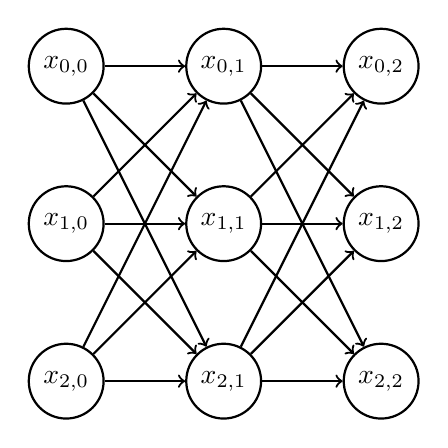
\begin{tikzpicture}[node distance={20mm}, thick, main/.style = {draw, circle}]
				\node[main] (0) {$x_{0,0}$};
				\node[main] (1) [below of=0]{$x_{1,0}$};
				\node[main] (2) [below of=1]{$x_{2,0}$};

				\node[main] (3) [right of=0]{$x_{0,1}$};
				\node[main] (4) [below of=3]{$x_{1,1}$};
				\node[main] (5) [below of=4]{$x_{2,1}$};

				\node[main] (6) [right of=3]{$x_{0,2}$};
				\node[main] (7) [below of=6]{$x_{1,2}$};
				\node[main] (8) [below of=7]{$x_{2,2}$};

				\draw[->] (0) -- (3);
				\draw[->] (0) -- (4);
				\draw[->] (0) -- (5);

				\draw[->] (1) -- (3);
				\draw[->] (1) -- (4);
				\draw[->] (1) -- (5);

				\draw[->] (2) -- (3);
				\draw[->] (2) -- (4);
				\draw[->] (2) -- (5);

				\draw[->] (3) -- (6);
				\draw[->] (3) -- (7);
				\draw[->] (3) -- (8);

				\draw[->] (4) -- (6);
				\draw[->] (4) -- (7);
				\draw[->] (4) -- (8);

				\draw[->] (5) -- (6);
				\draw[->] (5) -- (7);
				\draw[->] (5) -- (8);

			\end{tikzpicture}
			\caption[]{The initial graph}
			\label{figure:graph}
		\end{figure}
		Where the columns represent the words in $\mathbf{w}$ and the rows represent different tags.
		We use the algorithm from the script:\\
		\begin{algorithm}[H]
			\SetAlgoLined
			\caption{Forward pass}
			\label{algorithm:forward}
			$\beta(\mathbf{w}, t_0) = 1$\\
			\For{$n = 1 \to N$}{
				$\beta(\mathbf{w}, t_n) = \sum_{t_{n-1} \in \mathcal{T}} \exp(\score{\langle t_{n-1}}{t_n\rangle}) \otimes \beta(\mathbf{w}, t_{n-1})$
			}
		\end{algorithm}
		When we now lift the CRF into the expectation semiring, the forward propagation algorithm changes to:\\
		\begin{algorithm}[H]
			\SetAlgoLined
			\caption{Forward pass}
			\label{algorithm:forward_semi}
			$\beta(\mathbf{w}, t_0) = \langle 1, 0 \rangle$\\
			\For{$n = 1 \to N$}{
				$\beta(\mathbf{w}, t_n) = \oplus_{t_{n-1} \in \mathcal{T}} \langle w, -w \log w \rangle \otimes \beta(\mathbf{w}, t_{n-1})$
			}
		\end{algorithm}
		Where $w = \exp(\score{\langle t_n}{t_{n+1}\rangle})$.\\
		The output of the forward algorithm lifted into the semiring will yield:\\
		\begin{align}
			\bigoplus_{t_{1:N} \in T^{n}} \overset{N}{\bigotimes_{n=1}} \langle w, -w \log w \rangle
		\end{align}
		We want to show that the result of the forward propagation lifted in the semiring is the same as the unnormalized Entropy:
		\begin{align}
			H_u(T_{w}) & = -\sum_{\mathbf{t} \in \mathcal{T}^N} \exp(score_{\boldsymbol{\theta}} (\mathbf{t},\boldsymbol{w})) score_{\boldsymbol{\theta}} (\mathbf{t},\boldsymbol{w}) \label{eq:1b_to_show} \\
		\end{align}
		We show this by induction. Starting with the base case where $N = 1$:\\
		\begin{align}
			\bigoplus_{t_{1} \in T^{1}} \overset{1}{\bigotimes_{n=1}} \langle w, -w \log w \rangle & = \bigoplus_{t_{1} \in T^{1}} \langle \exp(\score{t_0}{t_1}),                     \\
			                                                                                       & \qquad -\exp(\score{t_0}{t_1}) \log(\exp(\score{t_0}{t_1})) \rangle               \\
			                                                                                       & = \bigoplus_{t \in T} \biggl< \exp(\sscore{t}),                         \nonumber \\
			                                                                                       & \qquad  -\exp(\sscore{t}) \log(\exp(\sscore{t})) \biggr>                          \\
			                                                                                       & = \biggl< \sum_{t \in T} \exp(\sscore{t}),                              \nonumber \\
			                                                                                       & \qquad -\sum_{t \in T} \exp(\sscore{t}) \log(\exp(\sscore{t})) \biggr>
		\end{align}
		Our induction hypothesis is the following:\\
		\begin{align}
			\bigoplus_{t_{1:i} \in T^{i}} \overset{i}{\bigotimes_{n=1}} \langle w, -w \log w \rangle = \left\langle \sum_{t \in T^{i}} \exp(\sscore{t}), -\sum_{t \in T^{i}} \exp(\sscore{t}) \log(\exp(\sscore{t})) \right\rangle
		\end{align}
		Meaning we assume that $\beta(\mathbf{w}, t_i)$ corresponds to the unnormalized entropy of all sequences of lenght $i$.\\
		Now we proceed with the induction step, where $i \rightarrow i + 1$:\\
		\begin{align}
			 & \bigoplus_{t_{1:i+1} \in T^{i+1}} \overset{i+1}{\bigotimes_{n=1}} \langle w, -w \log w \rangle \nonumber                                                                       \\ & = \bigoplus_{t_{1:i+1} \in T}  \left( \bigoplus_{t_{1:i} \in T^{i}} \overset{i}{\bigotimes_{n=1}} \langle w, -w \log w \rangle \right) \otimes \langle w, -w \log(w) \rangle \\
			 & \overset{\text{I.H.}}{=} \bigoplus_{t_{1:i+1} \in T} \left\langle \sum_{t \in T^{i}} \exp(\sscore{t}), -\sum_{t \in T^{i}} \exp(\sscore(t)) \sscore{t} \right\rangle \nonumber \\
			 & \otimes \left\langle \exp(\score{t_i}{t_{i+1}}), -\exp(\score{t_i}{t_{i+1}}) \score{t_i}{t_{i+1}}\right\rangle \label{eq:after_ih}
		\end{align}
		We will now analyze both parts of the semiring separately:
		\begin{align}
			 & \left(\sum_{t \in T^{i}} \exp(\sscore{t}) \right) \exp(\score{t_i}{t_{i+1}})                \\
			 & = \sum_{t \in T^{i}} \exp(\sscore{t}) + \score{t_i}{t_{i+1}}               \label{eq:semil}
		\end{align}
		And the second part:
		\begin{align}
			 & \left( \sum_{t \in T^{i}} \exp(\sscore{t}) \right) -\exp(\score{t_i}{t_{i+1}}) \score{t_i}{t_{i+1}} \nonumber                   \\
			 & \quad + \left( -\sum_{t \in T^{i}} \exp(\sscore(t)) \sscore{t} \right) \exp(\score{t_i}{t_{i+1}})                               \\
			 & = -\sum_{t \in T^{i}} \exp(\sscore{t} + \score{t_i}{t_{i+1}}) \score{t_i}{t_{i+1}} \nonumber                                    \\
			 & \quad -\left( \sum_{t \in T^{i}} \exp(\sscore(t)) \sscore{t} \right) \exp(\score{t_i}{t_{i+1}})                                 \\
			 & = -\sum_{t \in T^{i}} \exp(\sscore{t} + \score{t_i}{t_{i+1}}) \score{t_i}{t_{i+1}} \nonumber                                    \\
			 & \quad - \sum_{t \in T^{i}} \exp(\sscore{t} + \score{t_i}{t_{i+1}}) \sscore{t}                                                   \\
			 & = -\sum_{t \in T^{i}} \exp(\sscore{t} + \score{t_i}{t_{i+1}}) \left( \sscore{t} + \score{t_i}{t_{i+1}} \right) \label{eq:semir}
		\end{align}
		We can now combine the two parts to get with \cref{eq:after_ih}:
		\begin{align}
			 & \bigoplus_{t_{1:i+1} \in T} \left\langle \sum_{t \in T^{i}} \exp(\sscore{t}), -\sum_{t \in T^{i}} \exp(\sscore(t)) \sscore{t} \right\rangle \nonumber               \\
			 & \quad \otimes \left\langle \exp(\score{t_i}{t_{i+1}}), -\exp(\score{t_i}{t_{i+1}}) \score{t_i}{t_{i+1}}\right\rangle                                                \\
			 & \overset{\text{def. } \otimes}{=} \bigoplus_{t_{1:i+1} \in T} \biggl\langle \left(\sum_{t \in T^{i}} \exp(\sscore{t}) \right) \exp(\score{t_i}{t_{i+1}}), \nonumber \\
			 & \quad \left( \sum_{t \in T^{i}} \exp(\sscore{t}) \right) -\exp(\score{t_i}{t_{i+1}}) \score{t_i}{t_{i+1}} \nonumber                                                 \\
			 & \quad + \left( -\sum_{t \in T^{i}} \exp(\sscore(t)) \sscore{t} \right) \exp(\score{t_i}{t_{i+1}}) \biggr\rangle                                                     \\
			 & \overset{\cref{eq:semil}}{=} \bigoplus_{t_{1:i+1} \in T} \biggl\langle \sum_{t \in T^{i}} \exp(\sscore{t}) + \score{t_i}{t_{i+1}}, \nonumber                        \\
			 & \quad \left( \sum_{t \in T^{i}} \exp(\sscore{t}) \right) -\exp(\score{t_i}{t_{i+1}}) \score{t_i}{t_{i+1}} \nonumber                                                 \\
			 & \quad + \left( -\sum_{t \in T^{i}} \exp(\sscore(t)) \sscore{t} \right) \exp(\score{t_i}{t_{i+1}}) \biggr\rangle                                                     \\
			 & \overset{\cref{eq:semir}}{=} \bigoplus_{t_{1:i+1} \in T} \biggl\langle \sum_{t \in T^{i}} \exp(\sscore{t}) + \score{t_i}{t_{i+1}}, \nonumber                        \\
			 & \quad -\sum_{t \in T^{i}} \exp(\sscore{t} + \score{t_i}{t_{i+1}}) \left( \sscore{t} + \score{t_i}{t_{i+1}} \right) \biggr\rangle                                    \\
			 & \overset{\text{def. } \oplus}{=} \biggl\langle \sum_{t_{i+1} \in T} \sum_{t \in T^{i}} \exp(\sscore{t}) + \score{t_i}{t_{i+1}}, \nonumber                           \\
			 & \quad \sum_{t_{i+1} \in T} \sum_{t \in T^{i}} \exp(\sscore{t} + \score{t_i}{t_{i+1}}) \left( \sscore{t} + \score{t_i}{t_{i+1}} \right) \biggr\rangle                \\
			 & = \left\langle \sum_{t \in T^{i+1}} \exp(\sscore{t}), -\sum_{t \in T^{i+1}} \exp(\sscore{t}) \sscore{t} \right\rangle
		\end{align}
		Which concludes our induction proof and we have shown that \cref*{eq:1b_to_show} holds.
		% \begin{align}	
		% 	 & \bigoplus_{t_{1:N} \in T^{n}} \overset{N}{\bigotimes_{n=1}} \langle w, -w \log w \rangle                                                                                                                                                                                        \\
		% 	 & = \bigoplus_{t_{1:N-1} \in T^{N-1}} \bigoplus_{t_n \in T} \overset{N}{\bigotimes_{n=1}} \langle w, -w \log w \rangle                                                                                                                                                            \\
		% 	 & = \bigoplus_{t_{1:N-1} \in T^{N-1}} \overset{N-1}{\bigotimes_{n=1}} \langle \exp(\score{t_{n-1}}{t_n}), -\exp(\score{t_{n-1}}{t_n}) \log(\exp(\score{t_{n-1}}{t_n})) \rangle \nonumber                                                                                          \\
		% 	 & \qquad \otimes \bigoplus_{t_{N} \in T} \langle \exp(\score{t_{N-1}}{t_N}), -\exp(\score{t_{N-1}}{t_N}) \log(\exp(\score{t_{N-1}}{t_N})) \rangle                                                                                                                                 \\
		% 	 & = \bigoplus_{t_{1} \in T} \left\langle \exp(\score{t_0}{t_1}), -\exp(\score{t_0}{t_1}) \log(\exp(\score{t_0}{t_1})) \right\rangle \nonumber                                                                                                                                     \\
		% 	 & \qquad \otimes \bigoplus_{t_{2} \in T} \left\langle \exp(\score{t_1}{t_2}), -\exp(\score{t_1}{t_2}) \log(\exp(\score{t_1}{t_2})) \right\rangle \nonumber                                                                                                                        \\
		% 	 & \qquad \otimes \cdots \nonumber                                                                                                                                                                                                                                                 \\
		% 	 & \qquad \otimes \bigoplus_{t_{N} \in T} \left\langle \exp(\score{t_{N-1}}{t_N}), -\exp(\score{t_{N-1}}{t_N}) \log(\exp(\score{t_{N-1}}{t_N})) \right\rangle \nonumber                                                                                                            \\
		% 	 & = \biggr< \sum_{\mathbf{t} \in \mathcal{T}^N} \exp(score_{\boldsymbol{\theta}} (\mathbf{t},\boldsymbol{w})), -\sum_{\mathbf{t} \in \mathcal{T}^N} \exp(score_{\boldsymbol{\theta}} (\mathbf{t},\boldsymbol{w})) score_{\boldsymbol{\theta}} (\mathbf{t},\boldsymbol{w}) \biggr>
		% \end{align}
	\end{subquestion}
	\begin{subquestion}
		We want to prove:\\
		\begin{align}
			H(T_w) & = Z(\boldsymbol{w})^{-1} H_U(T) + \log(Z(\boldsymbol{w})
		\end{align}
		\begin{align}
			H(T_w) & = -\sum_{t \in T^{N}} p(t \:|\: w) \cdot \log(p(t \:|\: w))                                                                                                         &  & \text{(def. H)} \\
			       & = -\sum_{t \in T^{N}} \frac{\exp(\sscore{t})}{Z(\boldsymbol{w})} \log \left( \frac{\exp(\sscore{t})}{\sum_{t' \in T^N} \exp(\sscore{t'})} \right)                   &  & \text{(def. p)} \\
			       & = -\sum_{t \in T^{N}} \frac{\exp(\sscore{t})}{Z(\boldsymbol{w})} \log \left( \frac{\exp(\sscore{t})}{Z(\boldsymbol{w})} \right)                                                          \\
			       & = -\sum_{t \in T^{N}} \frac{\exp(\sscore{t})}{Z(\boldsymbol{w})} (\sscore{t} - \log Z(\boldsymbol{w}))                                                                                   \\
			       & = -\sum_{t \in T^{N}} \frac{\exp(\sscore{t}) \sscore{t} - \exp(\sscore{t}) \log Z(\boldsymbol{w}))}{Z(\boldsymbol{w})}                                                                   \\
			       & = -\sum_{t \in T^{N}} \frac{\exp(\sscore{t}) \sscore{t}}{Z(\boldsymbol{w})} + \sum_{t \in T^{N}} \frac{\exp(\sscore{t}) \log Z(\boldsymbol{w}))}{Z(\boldsymbol{w})}                      \\
			       & = H_U(T_{\boldsymbol{w}}) Z(\boldsymbol{w})^{-1}  + \frac{\log(Z(\boldsymbol{w}))}{Z(\boldsymbol{w})} \sum_{t \in T^{N}} \exp(\sscore{t})                                                \\
			       & = H_U(T_{\boldsymbol{w}}) Z(\boldsymbol{w})^{-1}  + \log(Z(\boldsymbol{w}))                                                                                                              \\
		\end{align}
	\end{subquestion}
\end{question}
\end{document}

%%% Local Variables:
%%% mode: latex
%%% TeX-master: t
%%% End: